\documentclass[t, 11pt, xcolor=dvipsnames]{beamer}
\usepackage{textcomp}
\usepackage{mathtools}
\usepackage{pdfpages}
\usepackage{graphicx}
\usepackage{tikz}
\usepackage{multimedia}
\usepackage{transparent}
\usetikzlibrary{calc}

%%%%%%%%%%%%%%%%%%%%%%%%%%%%%%%%%%%%%%%%%%%%%%%%%%%%%%%%%%%%
% Useful things

% list
%% \begin{itemize}
%% \item List a
%% \item List b
%% \end{itemize}

% image
%% \begin{center}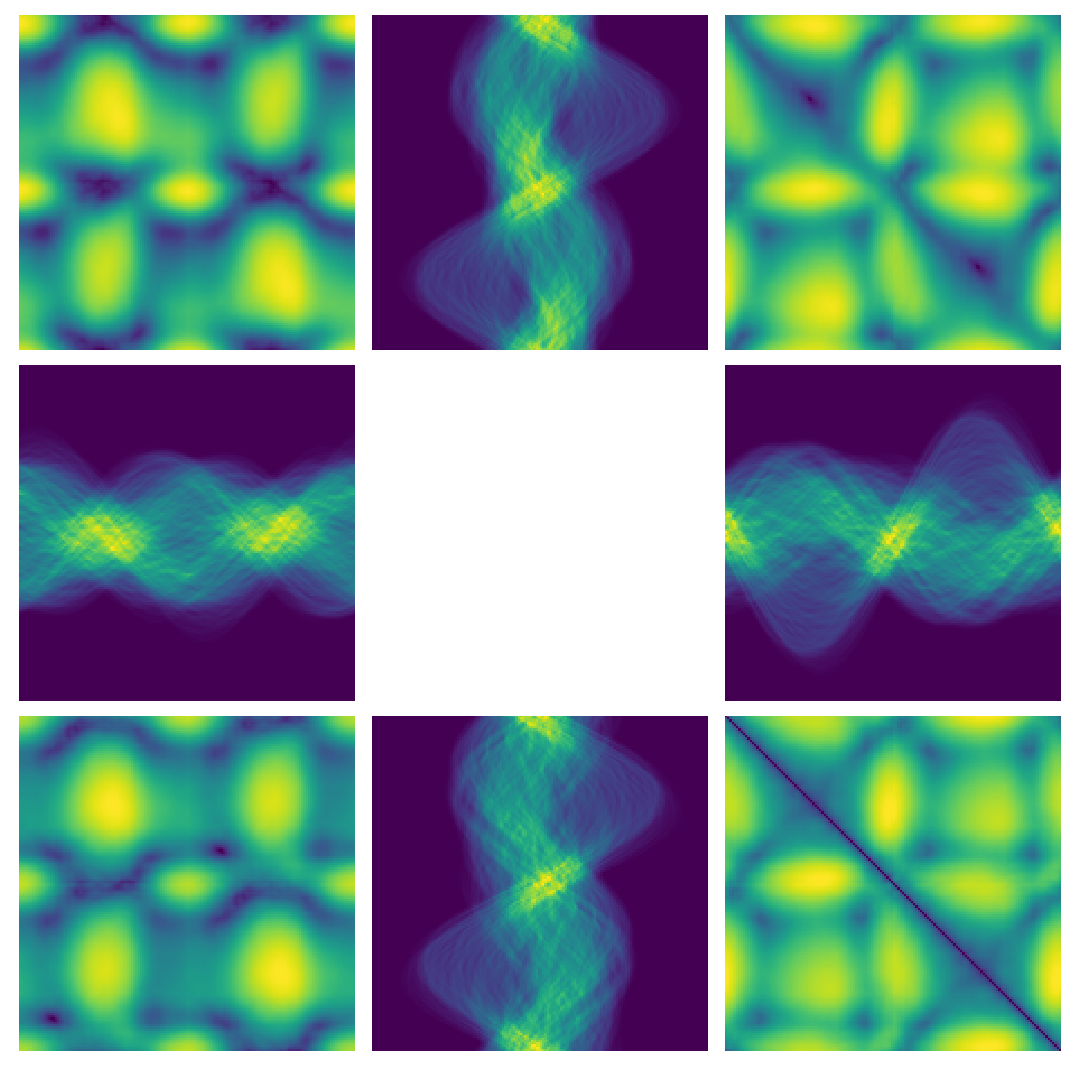
\includegraphics[width=0.45\textwidth]{images/Sinogram_3_comp.png}
%% \end{center}

% absolute position
%% \placetextbox[north west]{0.37}{0.33}{\setlength{\fboxsep}{0pt}\setlength{\fboxrule}{0.5pt}\fbox{absolute position1}}
%% \placetextbox[north west]{0.77}{0.33}{\setlength{\fboxsep}{0pt}\setlength{\fboxrule}{0.5pt}\fbox{absolute postion 2}}

% movie
%% \placetextbox[north west]{0.083}{0.30}{\movie[width=3.5cm,height=2cm,poster, externalviewer, loop]{\includegraphics[width=3.5cm]{movie_still.png}}{movie.webm}}
%%%%%%%%%%%%%%%%%%%%%%%%%%%%%%%%%%%%%%%%%%%%%%%%%%%%%%%%%%%%

%%%%%%%%%%%%%%%%%%%%%%%%%%%%%%%%%%%%%%%%%%%%%%%%%%%%%%%%%%%%
% absolute positioning of typeset material    
%%%%%%%%%%%%%%%%%%%%%%%%%%%%%%%%%%%%%%%%%%%%%%%%%%%%%%%%%%%%
\newcommand{\placetextbox}[4][center]{%
  % [#1]: box anchor: center (default) | 
  %                 south west | west | north west | north |
  %                 north east | east | south east | south | 
  %                 mid west | mid | mid east |
  %                 base west | base | base east 
  % #2: horizontal position (fraction of page width)
  % #3: vertical position (fraction of page height)
  % #4: content
  %
  \tikz[remember picture,overlay,x=\paperwidth,y=\paperheight]{%
    \node[anchor=#1,inner sep=0pt]
    at ($(current page.south west)+(#2,#3)$) {#4};
  }%
}
%%%%%%%%%%%%%%%%%%%%%%%%%%%%%%%%%%%%%%%%%%%%%%%%%%%%%%%%%%%%

\usetheme{Berlin}

% \usecolortheme[named=UBCblue]{structure}
% \usecolortheme[named=Mahogany]{structure} % Sample dvipsnames color
\definecolor{UBCblue}{rgb}{0.04706, 0.13725, 0.26667} % UBC Blue (primary)
\definecolor{UBCgrey}{rgb}{0.3686, 0.5255, 0.6235} % UBC Grey (secondary)

\definecolor{CLICbrown}{rgb}{0.438, 0.309, 0.313}
\definecolor{CLICorange}{rgb}{0.938, 0.660, 0.473}
\definecolor{CLICyellow}{rgb}{0.973, 0.938, 0.684}
\definecolor{CLICbg}{rgb}{0.113, 0.125, 0.129}
\definecolor{CLICfg}{rgb}{0.895, 0.895, 0.895}

%% \setbeamercolor{palette primary}{bg=CLICbrown,fg=white}
%% \setbeamercolor{palette secondary}{bg=CLICorange,fg=white}
%% \setbeamercolor{palette tertiary}{bg=CLICyellow,fg=white}
%% % \setbeamercolor{palette quaternary}{bg=CLICbrown,fg=white}
%% \setbeamercolor{structure}{fg=CLICfg} % itemize, enumerate, etc
%% \setbeamercolor{structure}{bg=CLICbg} % itemize, enumerate, etc
%% \setbeamercolor{section in toc}{fg=CLICfg} % TOC sections

%% % Override palette coloring with secondary
%% \setbeamercolor{subsection in head/foot}{bg=UBCgrey,fg=white}
%% \setbeamercolor{normal text}{bg=CLICfg, fg=CLICfg}
%% \setbeamercolor{background canvas}{bg=CLICbg}


\def\liketitle#1{%
{\usebeamerfont{frametitle}\usebeamercolor[fg]{structure}%
\begin{flushleft}%
\vspace{-\baselineskip}% Cometic correction for space introduced by flushleft
#1\par
\end{flushleft}%
\vspace{-\baselineskip}% Cosmetic correction for space introduced by flushleft
}%
\vspace{0.75\baselineskip}%
}
\logo{\makebox[0.7\paperwidth]{
\includegraphics[width=1cm,keepaspectratio]{images/Diamond.png}}} % Insert logo !XXXX
\date{March 23rd, 2020}
\author{Donovan Webb}
\institute{eBIC/University of Bath}
\titlegraphic{
\includegraphics[width=3cm]{images/Diamond.png}}
\titlegraphic{
\includegraphics[width=3cm]{images/Diamond.png}} % Insert logo !XXXX
\title{CLIC}
\subtitle{Common Lines Implied Clustering}

\AtBeginSection[]{
  \begin{frame}
  \vfill
  \centering
  \begin{beamercolorbox}[sep=8pt,center,shadow=false,rounded=false]{title}
    \usebeamerfont{title}\insertsectionhead\par%
  \end{beamercolorbox}
  \vfill
  \end{frame}
}

\begin{document}

\setbeamertemplate{navigation symbols}{}
\begin{frame}[plain]
  \maketitle
\end{frame}
\addtocounter{framenumber}{-1} % Don't count title slide !XXXX

\begin{frame}{Table of Contents}
  \tableofcontents[sectionstyle=show/show, hideallsubsections]
\end{frame}


\section{Single Lines}

\begin{frame}[fragile]{The Radon Transform}
 \begin{center}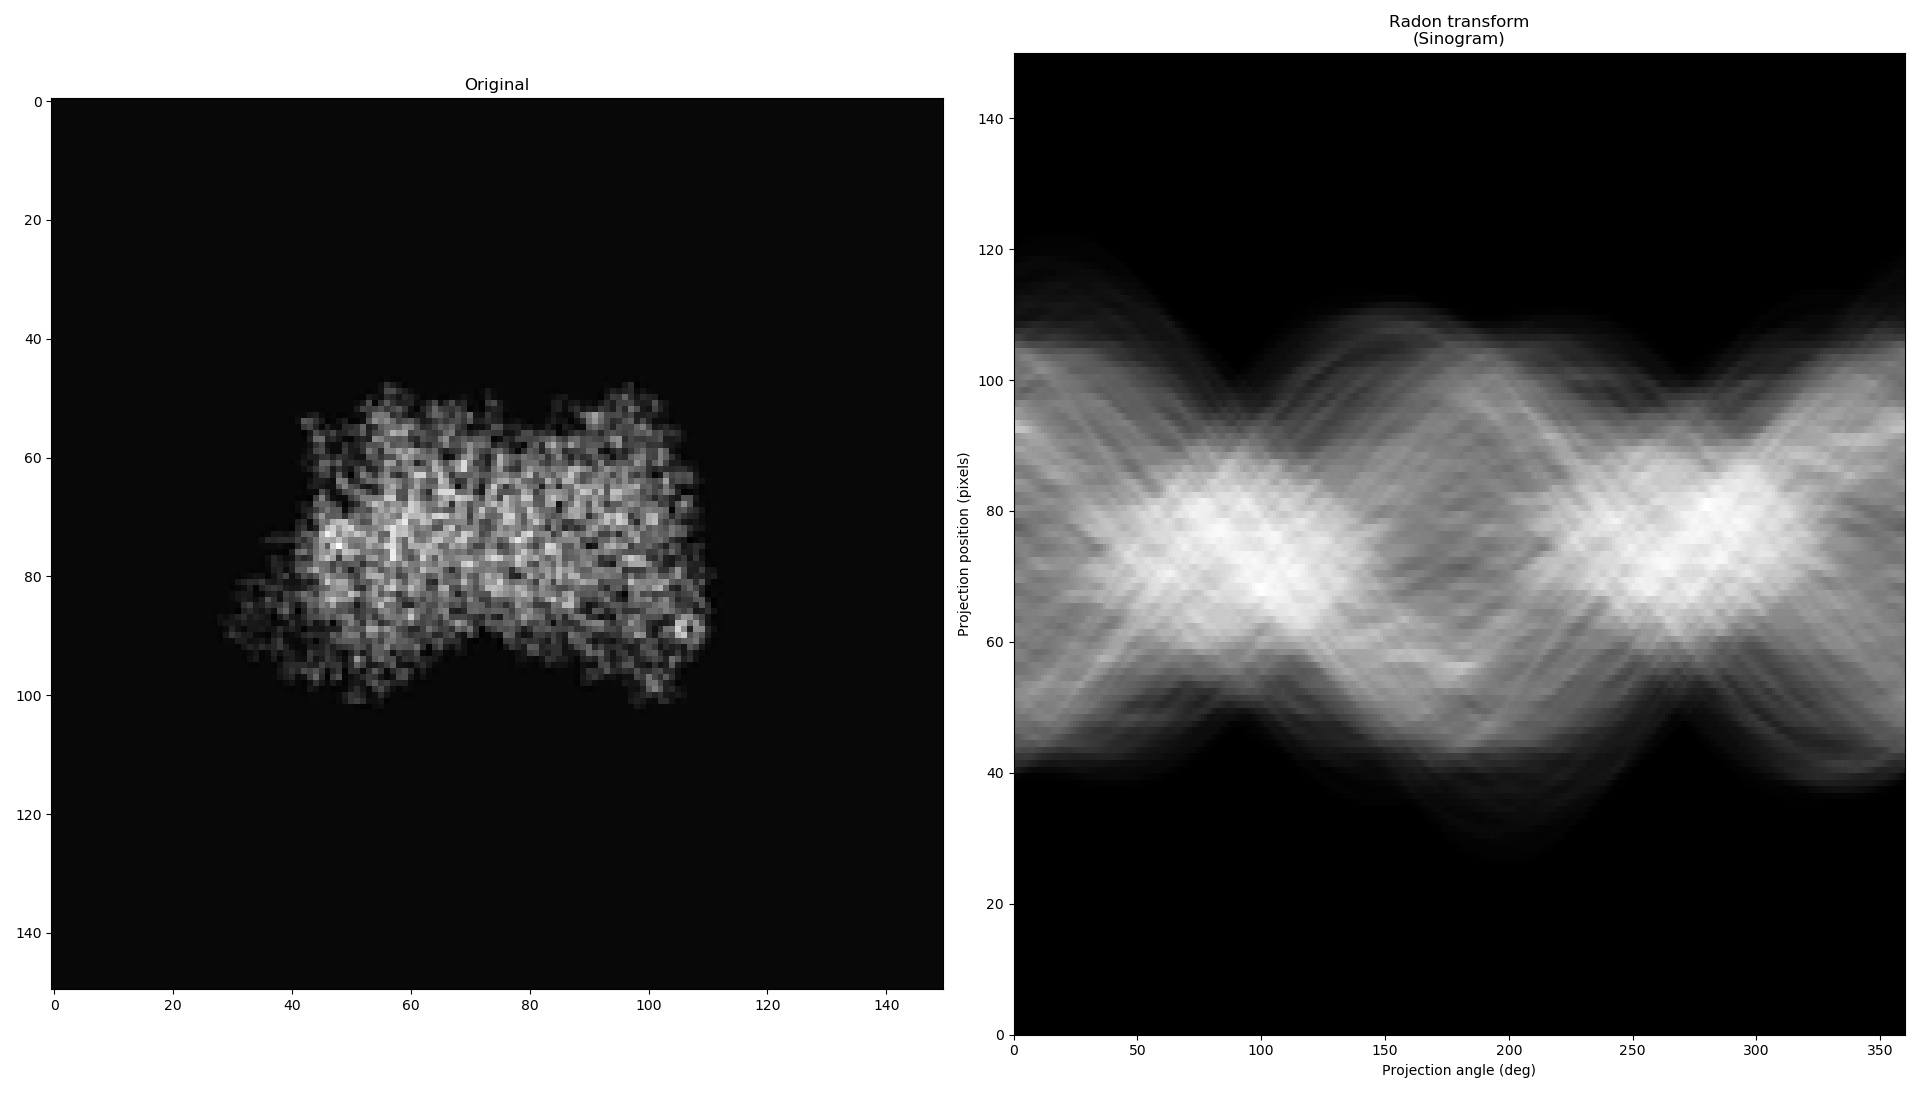
\includegraphics[width=0.9\textwidth]{images/Sinogram_Proj1.png}
    \end{center}
\vspace{-1em}
\end{frame}

\begin{frame}[fragile]{The Radon Transform}
 \only<1>{\begin{center}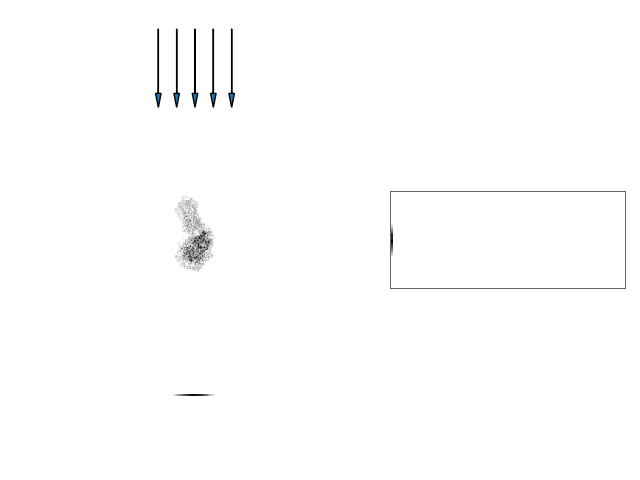
\includegraphics[width=0.85\textwidth]{images/sino_ani/sino_make_fr1.png}
    \end{center}}
 \only<2>{\begin{center}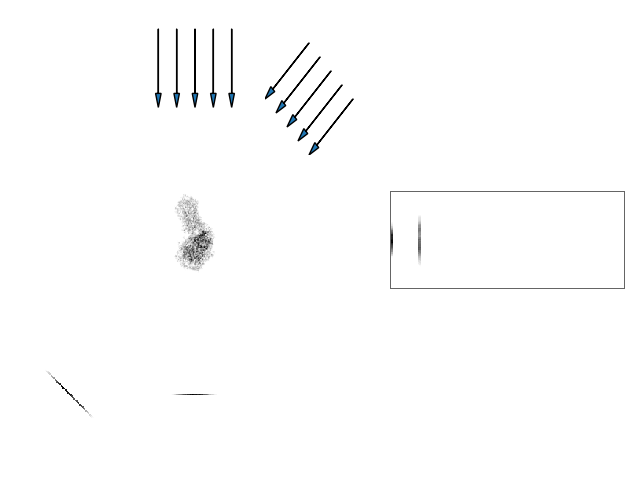
\includegraphics[width=0.85\textwidth]{images/sino_ani/sino_make_fr2.png}
    \end{center}}
 \only<3>{\begin{center}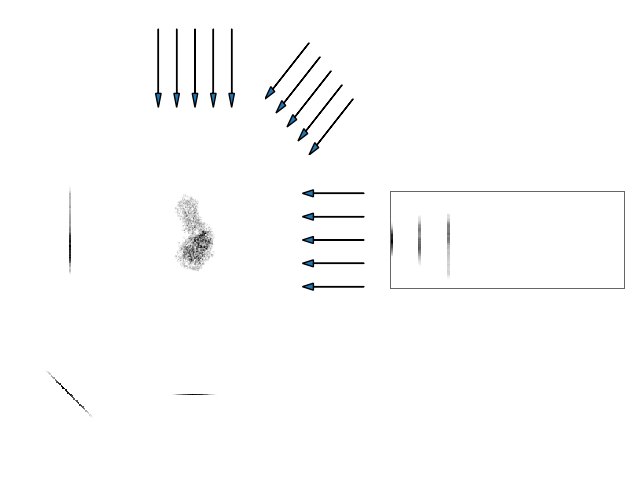
\includegraphics[width=0.85\textwidth]{images/sino_ani/sino_make_fr3.png}
    \end{center}}
 \only<4>{\begin{center}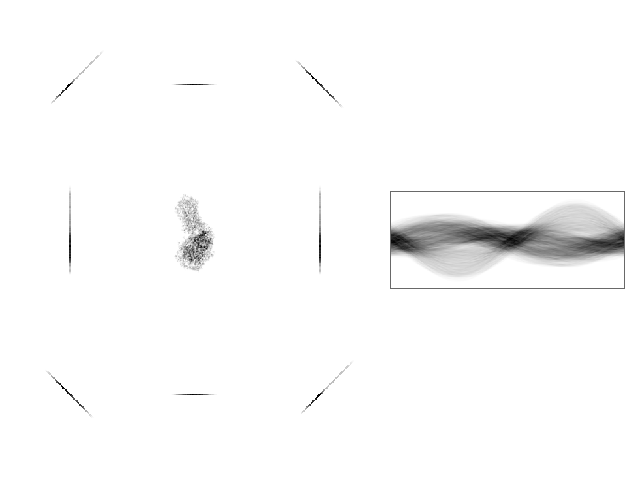
\includegraphics[width=0.85\textwidth]{images/sino_ani/sino_make_fr4.png}
    \end{center}}
\end{frame}

\begin{frame}[fragile]{Common Lines}
  \textbf{Two projections of the same 3D volume share at least one common line in the Radon transform}
 \begin{center}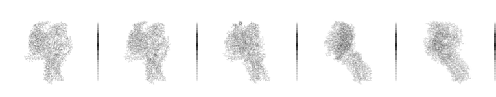
\includegraphics[width=0.85\textwidth]{images/common_line.png}
    \end{center}
 \begin{center}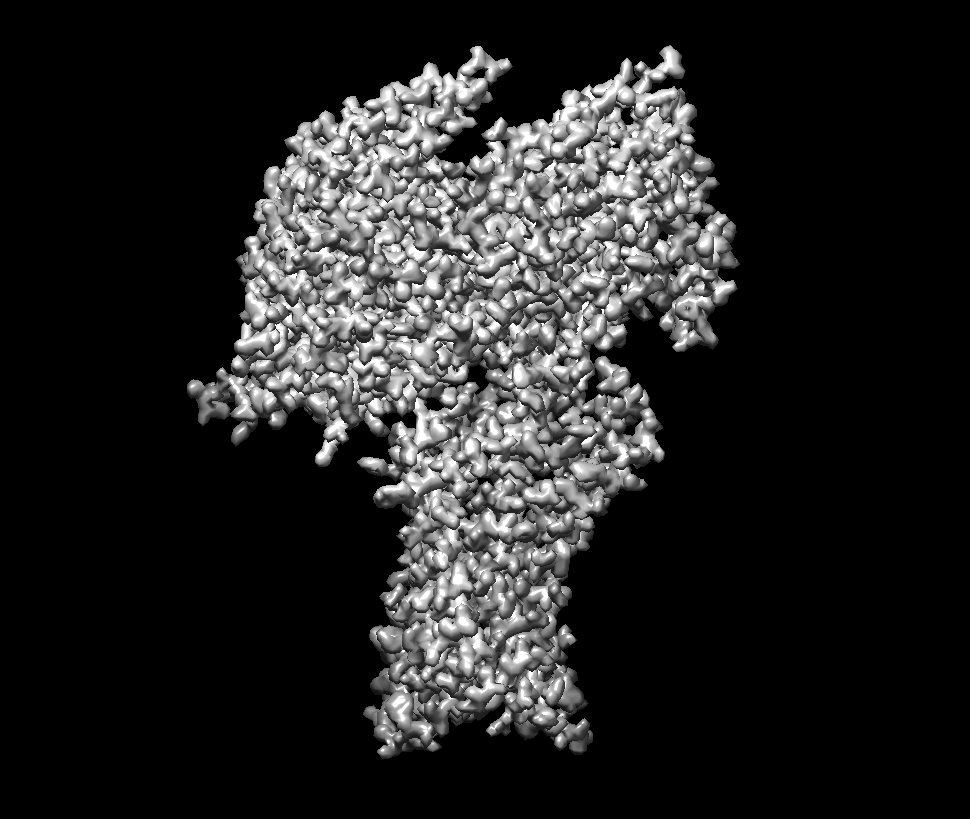
\includegraphics[width=0.35\textwidth]{images/3D_model.png}
    \end{center}
\end{frame}

\begin{frame}[fragile]{Common Lines}
  \centering\textbf{What about two different 3D volumes?}
 % Include new figure comparing lines from two models !XXXX
 \begin{center}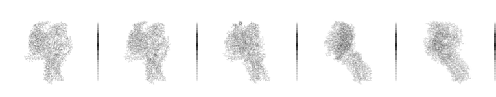
\includegraphics[width=0.85\textwidth]{images/common_line.png}
    \end{center}
 \begin{center}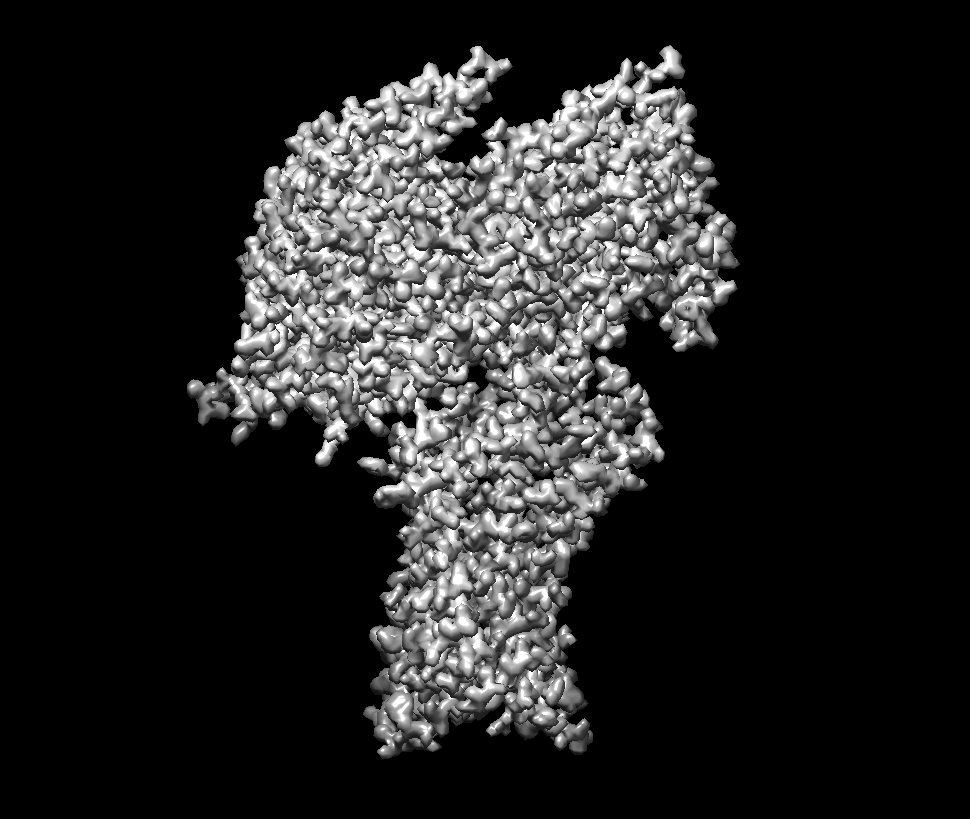
\includegraphics[width=0.35\textwidth]{images/3D_model.png}
    \end{center}
\end{frame}

\section{Finding Common Lines}

\begin{frame}[fragile]{Sinogram Cross Correlation}
  \centering\textbf{Finding the common line between two sinograms}
  \begin{center}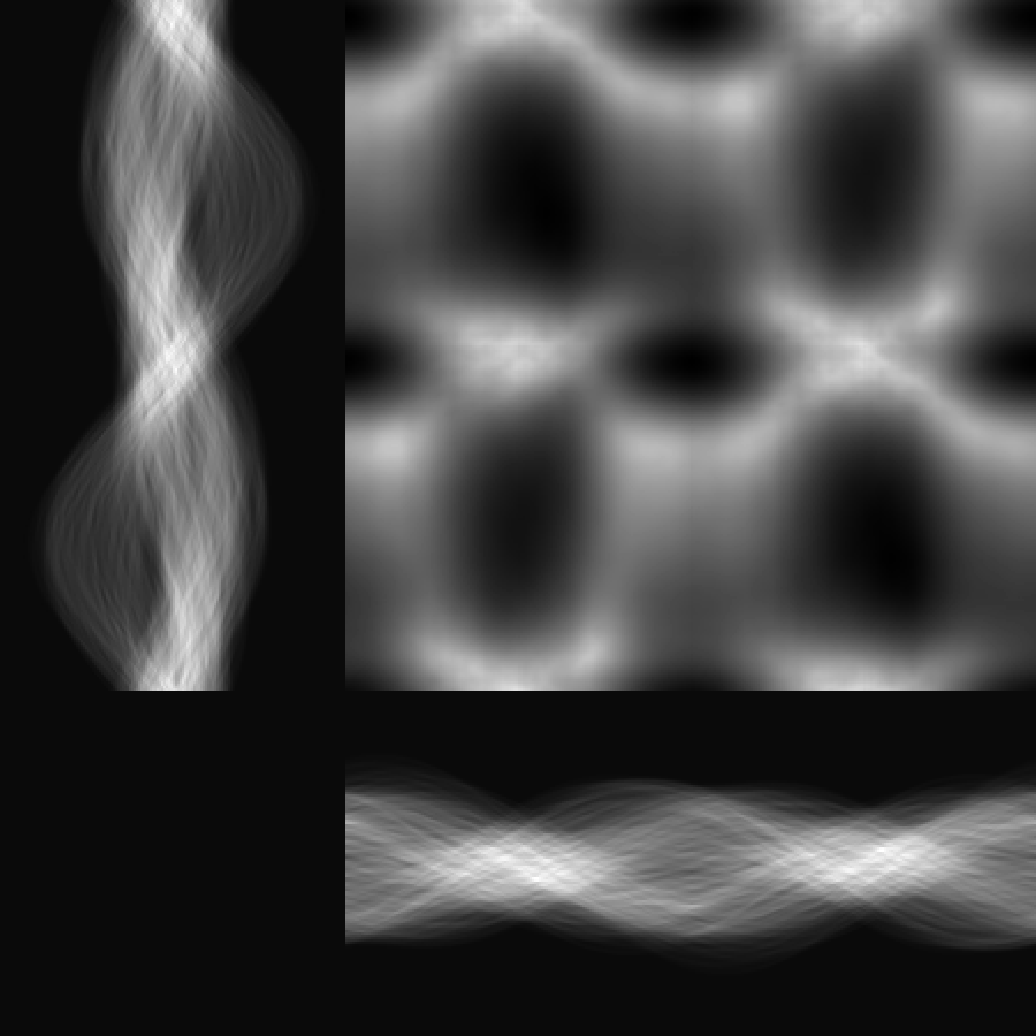
\includegraphics[width=0.7\textwidth]{images/2sin_comp.png}
    \end{center}
  \pause
  \centering\textbf{But what about N sinograms?} \\
  \pause
  \centering\textbf{What about N sinograms from a heterogenous dataset?}

\end{frame}


\begin{frame}[fragile]{Pipeline}
    \begin{itemize}
    \item Plot each line in high dimensional space % One pixel is one variable
    \item Find Euclidean Distances 
    \item Smaller distances mean better agreement
    \item Best match between two sinograms \textrightarrow{} Common line!
    \item Best scoring common lines \textrightarrow{} From the same model!
    \end{itemize}
    % Make this a flow chart !XXXX
    % Include graphic of points plotted in 2d space !XXXX

    \pause
    Slow.
    \pause
    Exhaustive.
    \pause
    Doesn't handle noise well.
\end{frame}

\begin{frame}[fragile]{Dimensional Reduction}
  \centering\textbf{Find features - Reduce noise}

  % Swiss roll explanation? !XXXX

  % Dimensional reduction can be used to lower influence of noise and try to find common features of data.
  % Manifold learning found to improve accuracy of common lines being chosen although more computationally expensive.
  % Plot 2D pca of sinogram !XXXX
  % and non-linear Iso map or lle !XXXX
  Linear \\
  PCA\\
  % Plot 2D of sinogram !XXXX

  Non-Linear \\
  LLE\\
  % Plot 2D of sinogram !XXXX
  Isomap \\
  % Plot 2D of sinogram !XXXX
  TSNE\\
  % Plot 2D of sinogram !XXXX
  UMAP\\
  % Plot 2D of sinogram !XXXX

\end{frame}

\begin{frame}[fragile]{Pipeline}
    \begin{itemize}
    \item Plot each line in high dimensional space % One pixel is one variable
    \item Apply dimensional reduction % One pixel is one variable
    \item Find Euclidean Distances 
    \item Smaller distances mean better agreement
    \item Best match between two sinograms \textrightarrow{} Common line!
    \item Best scoring common lines \textrightarrow{} From the same model!
    \end{itemize}
    % Make this a flow chart !XXXX
    % Include graphic of points plotted in 2d space !XXXX

    \pause
    But how do we assign clusters?
\end{frame}

\section{Clustering}
\begin{frame}{Can heterogenaity be sorted by looking at common lines?}
  % Figure of 2D representation of lines using TSNE. !XXXX
  Ground truth: Good seperatation between two classes - but discontinuous
  % Figures from update page
  %% yes, we can use the relationship between single lines from the same sinogram and from the same model.
  %% Cant use conventional clustering algorithms as cluster is not all spatially in the same place.
  %% We made our own based off of agglomerative method.
  %% For 800 (400 each from two classes) we get 100 \% success in clustering. Takes 20 minutes...
  %% For 800 (200 each from 4 classes, 2 classes very similar) we get  100\% success in clustering the differnt 3.
  %% In order to know where to cut the tree we look when a large jump occurs. - Two large groups merging

  %% Issues with clustering: Ctf, off centering, noise.
\end{frame}

\begin{frame}{Heirarchical clustering}
  % Insert fig !XXXX
\end{frame}

\begin{frame}[fragile]{Pipeline}
    \begin{itemize}
    \item Plot each line in high dimensional space % One pixel is one variable
    \item Apply dimensional reduction % One pixel is one variable
    \item Find Euclidean Distances 
    \item Smaller distances mean better agreement - Create score
    \item Heirarchical Clustering
    \item Cut tree to produce clusters
    \end{itemize}

    \pause
    Just a model left!
\end{frame}

\section{Reconstruction}

\begin{frame}[fragile]{Angular recovery from 3 Common lines}
  \textbf{Common line gives axis of rotation.}
  Three common lines gives 2 unique solutions for 3D orientation (One mirror of other)
  \only<1>{\begin{center}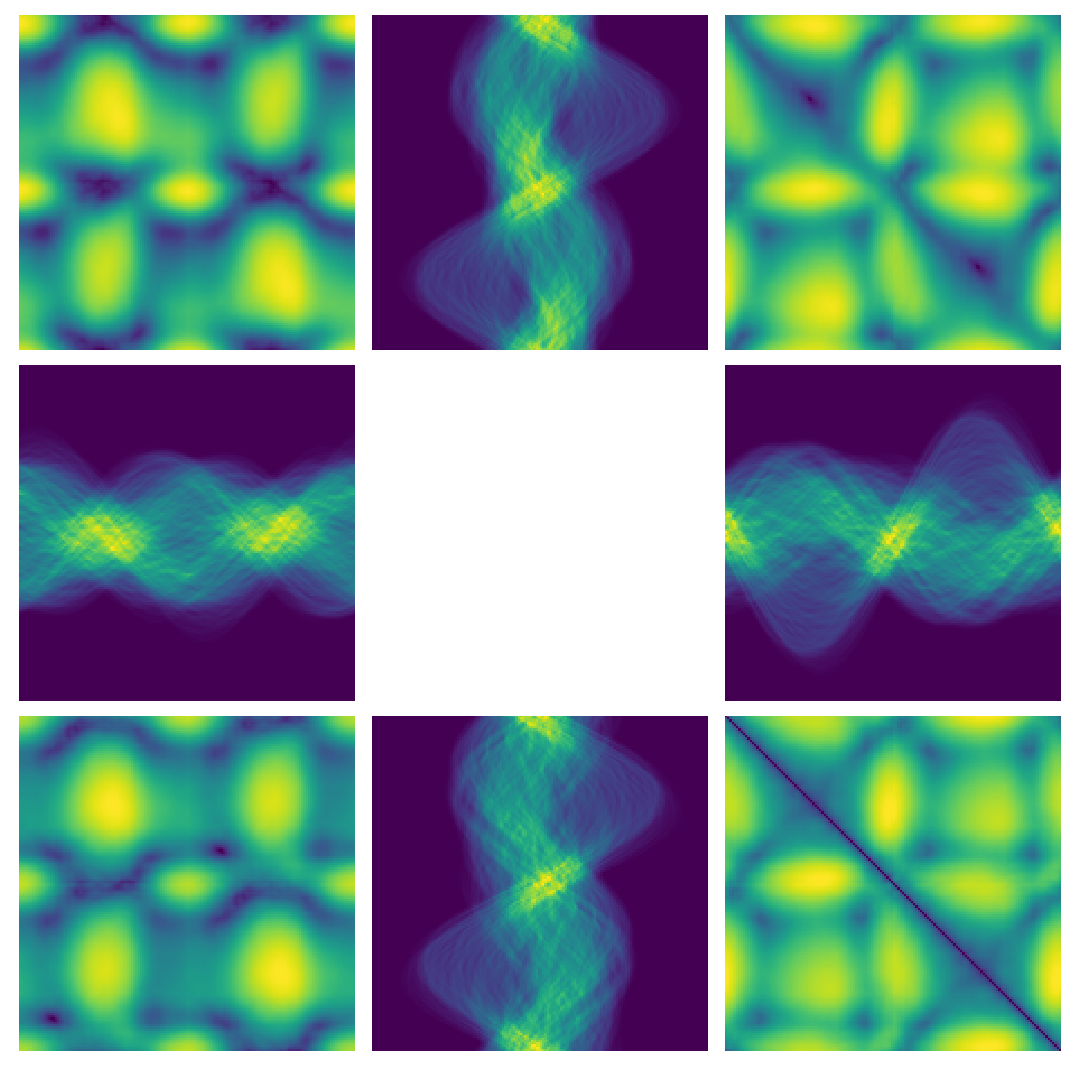
\includegraphics[width=0.45\textwidth]{images/Sinogram_3_comp.png}
    \end{center}}
  \only<2->{\begin{center}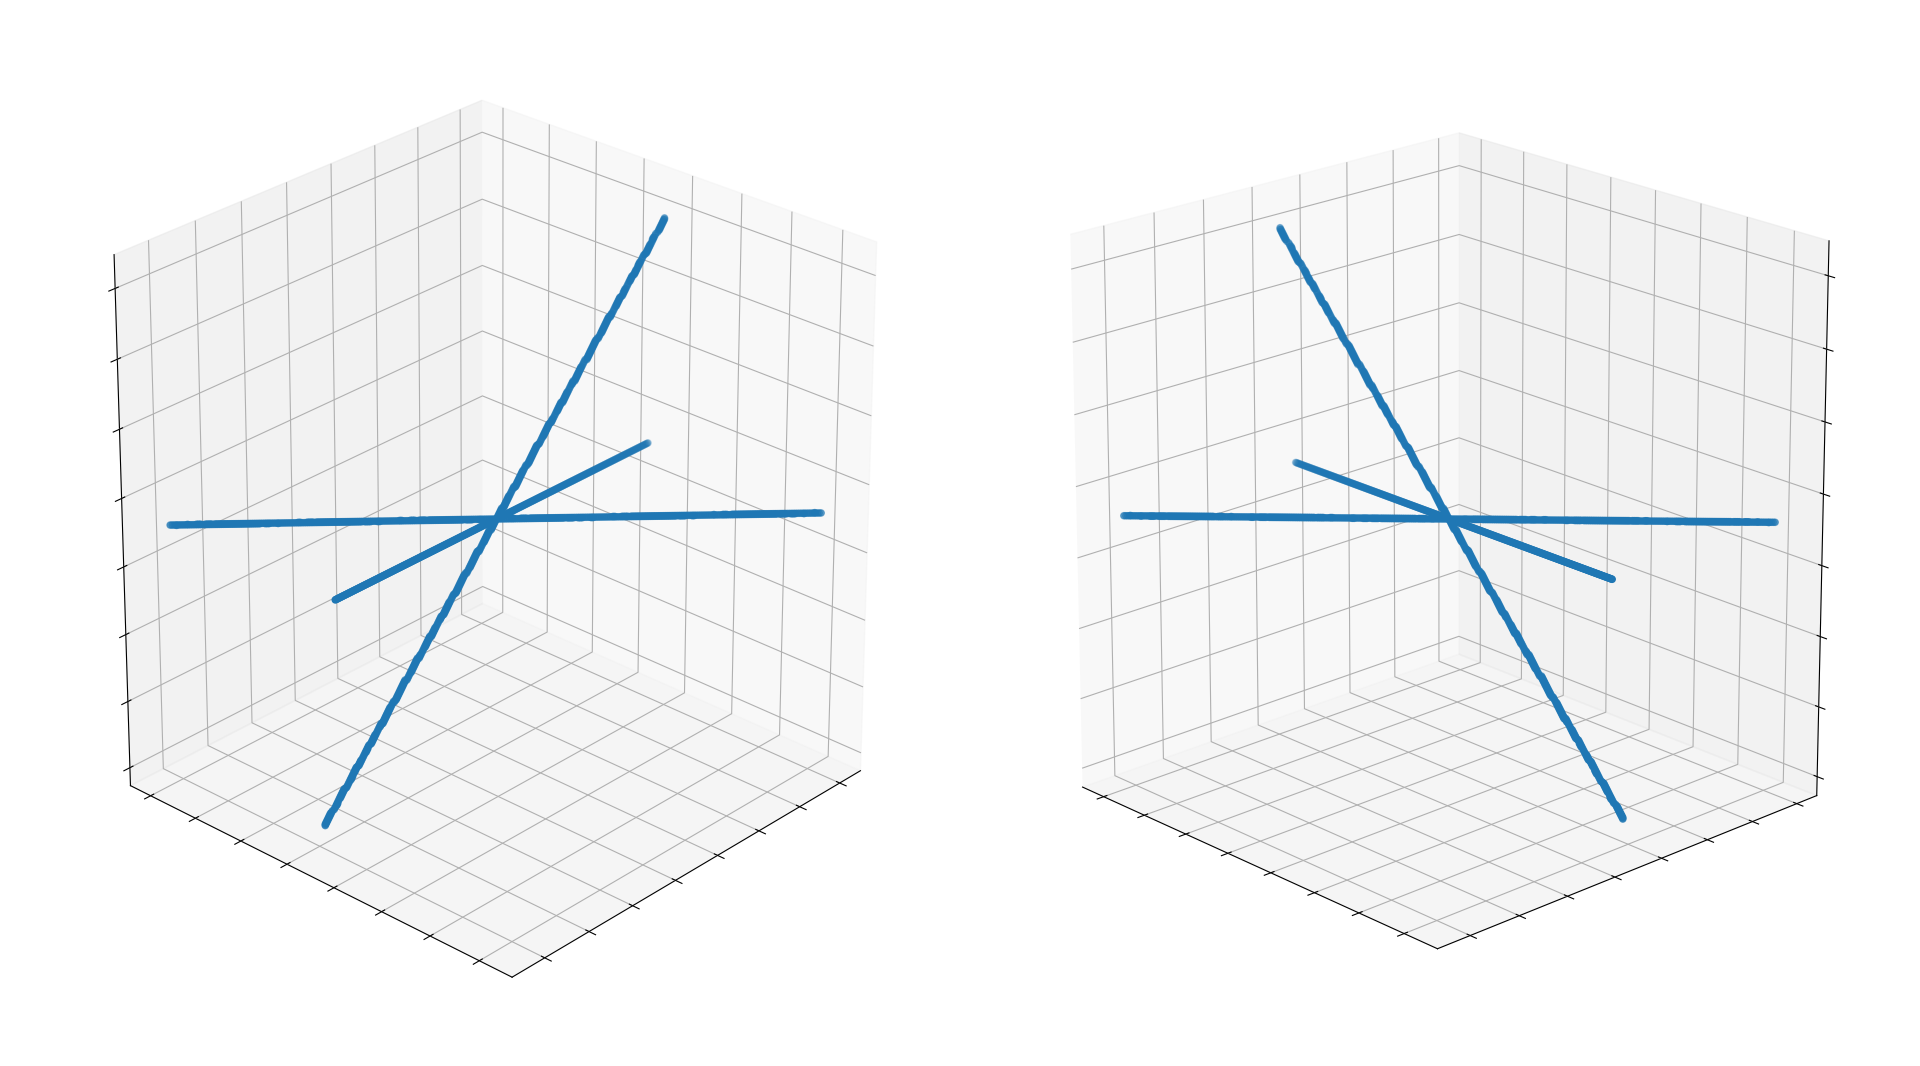
\includegraphics[width=0.801\textwidth]{images/vectors.png}
    \end{center}}
  \textit{\tiny{Angular Reconstitution: A Posteriori Assignment of Projection Directions for 3d Reconstruction. Van Heel 1987}}
  \only<3>{\placetextbox[north west]{0.34}{0.63}{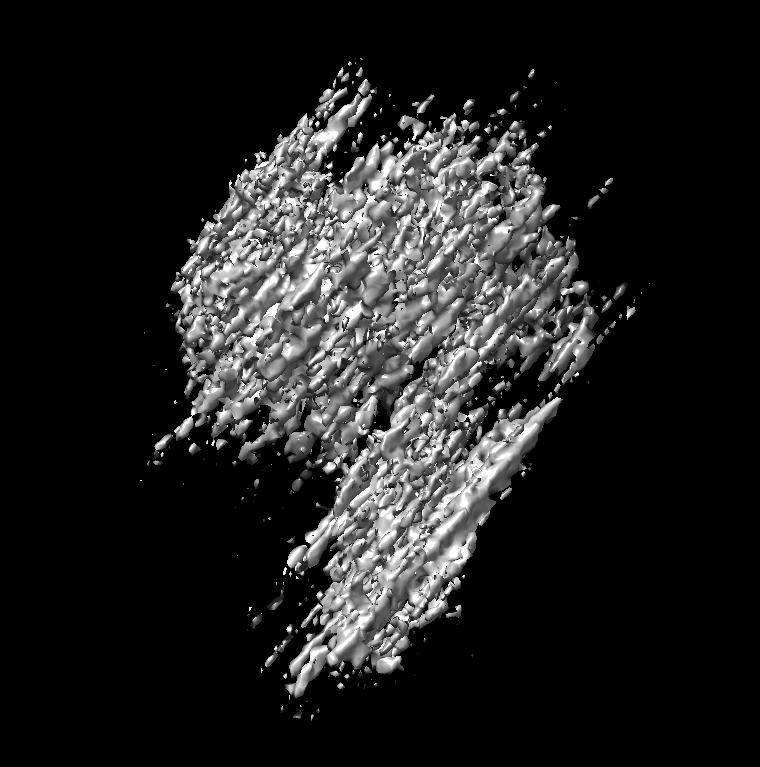
\includegraphics[width=0.4\linewidth]{images/3_line_model.png}}}
\end{frame}

\begin{frame}[fragile]{Eigenvector Relaxation}
  \small
  \textbf{Aim: Given all common lines $c$ for projections $P$, assign Rotation matrices $R$ for each $P$ to give greatest consensus volume.} \\
  \vspace{0.5em}
  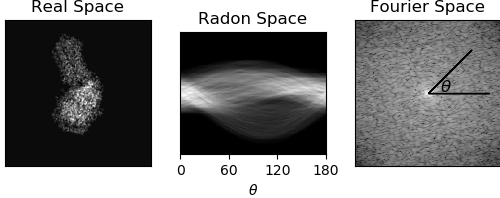
\includegraphics[width=0.45\textwidth]{images/radon_ft.png}
\vspace{-3.7em}
  \hspace*{3.2em}\vbox{\tiny{$$\hspace{15em}cij~=~(cos(\theta_{ij}),sin(\theta_{ij}),0),~cji~=~(cos(\theta_{ji}),sin(\theta_{ji}),0)~\quad~(1)$$}}

  \small
 \placetextbox[north west]{0.56}{0.45}{
  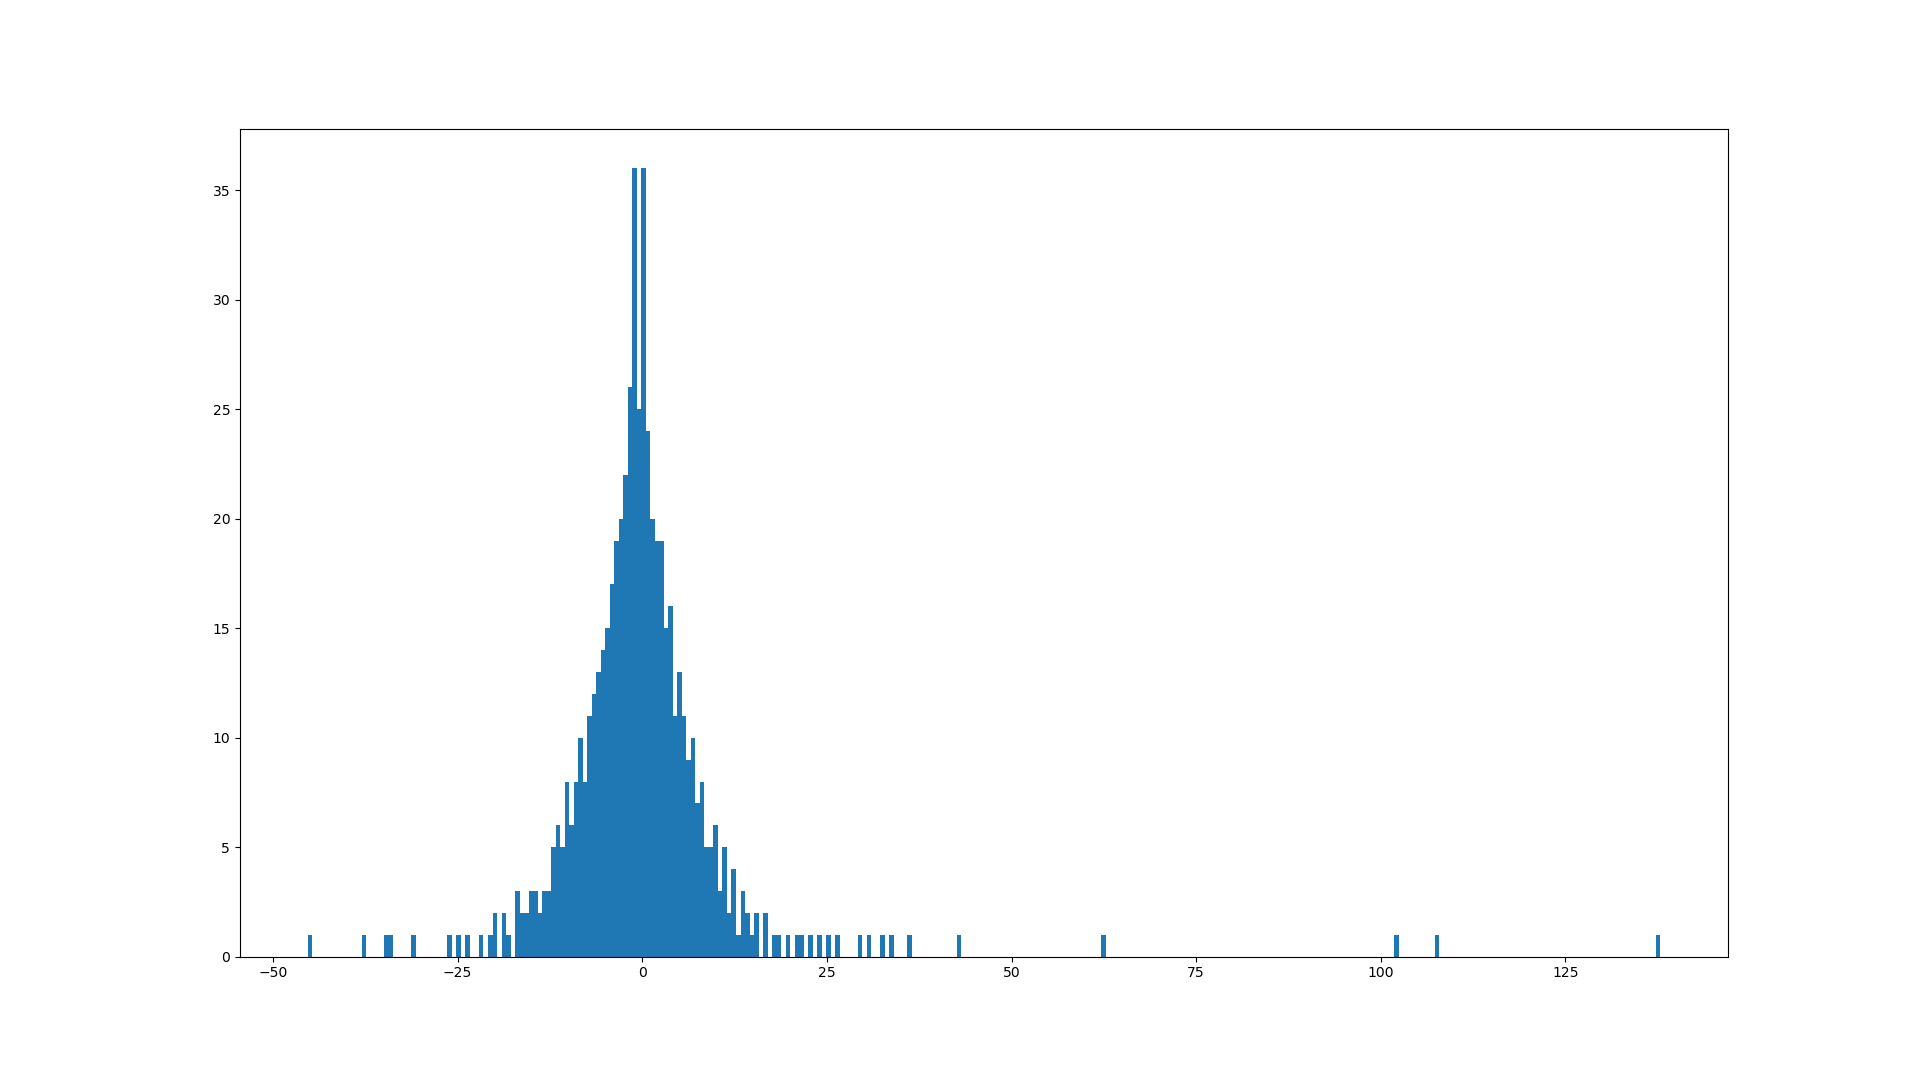
\includegraphics[width=0.55\textwidth]{images/eighist.png}} \\
  \vspace{1em}
  \hspace*{-2em}\vbox{$$max\sum_{i\ne j} R_ic_{ij} \cdot R_jc_{ji} \quad (2)$$}
  Maths*! Make large $(2N \times 2N)$ symmetric \\ matrix $S$. Can recover $R$ for each $P$ from \\ top 3 eigenvectors of $S$ that maximise (2)! \\
  
  \vspace{2em}

  \textit{\scalebox{0.5}{*Three Dimensional Structure Determination from Common Lines in Cryo-EM by Eigenvectors and Semidefinite Programming. A.Singer and Y.Shkolnisky}}
\end{frame}

\section{Full Pipeline}
\begin{frame}{}
  A full pipeline of the procedure.
  2d projs > 2d sins > 1d lines > TSNE > agglo > clusters > split into sep datasets > find common lines > eigenvector relaxation > Models
\end{frame}

\end{document}

%% \section{Reconstruction}
%% \subsection*{Too many Lines}
%% % \begin{frame}[fragile]{Voting}
%% %   Take all lines pairs under distance X
%% %   This gives multiple possible axis between the same two projections. Weight these according to distance and number of times they appear.
%% %   For each common line between two sinograms get more than 1 match so... vote which is best!
%% % \end{frame}

%% % \begin{frame}[fragile]{Overdetermined system}
%% %   % https://www.osapublishing.org/josaa/fulltext.cfm?uri=josaa-9-10-1749&id=64057
%% %   3 projections can satisfy geometrical constraints.
%% %   Problem when we add a fourth!
%% %   R = matrix
%% %   need 6 variables per projection.
%% %   Each pair of projection gives us 2 variables. 
%% %   2 N^2 vs 6N
%% %   if N = 3 then we have determined system
%% %   3 lines is all good for getting angular information back c.f. prev slide.
%% %   any more than 3 and we can get contradicting equations - system is overdetermined. we have N\^2 linear equations and only 6N variables (do proper maths)
%% %   Machine learning 3! how to fit. Least squares optimization not good as we have large number of misidentified lines and nonconvex! we also need to get proper rotation matrices at the end. This constraint leads to collapse to trivial solution 000. Need other approach.
%% % \end{frame}

